\chapter{Composizione del corpo stradale}

Si può procedere con la modellazione della sezione trasversale della strada. Il modello chiamato template si crea attraverso l'utilizzazione di modelli già esistenti nella libreria del programma Open Roads con l'aggiunta di elementi creati dall'utente. Per creare il template si utilizza il comando Corridors/Create Template. Il template utilizzato è quello denominato come $X_REV_5$ (\ref{Sezione tipo X}) a cui vengono apportate le modifiche necessarie, in particolare per quanto riguarda la lunghezza della corsia e della banchina, in modo da rispettare i criteri per le strade di tipo F extraurbana.
In particolare, la normativa, impone per una strada di tipo F una larghezza della corsia pari a 3,5 metri e consiglia un valore minimo di larghezza della banchina pari a 1 metro.

\begin{figure}[H]
    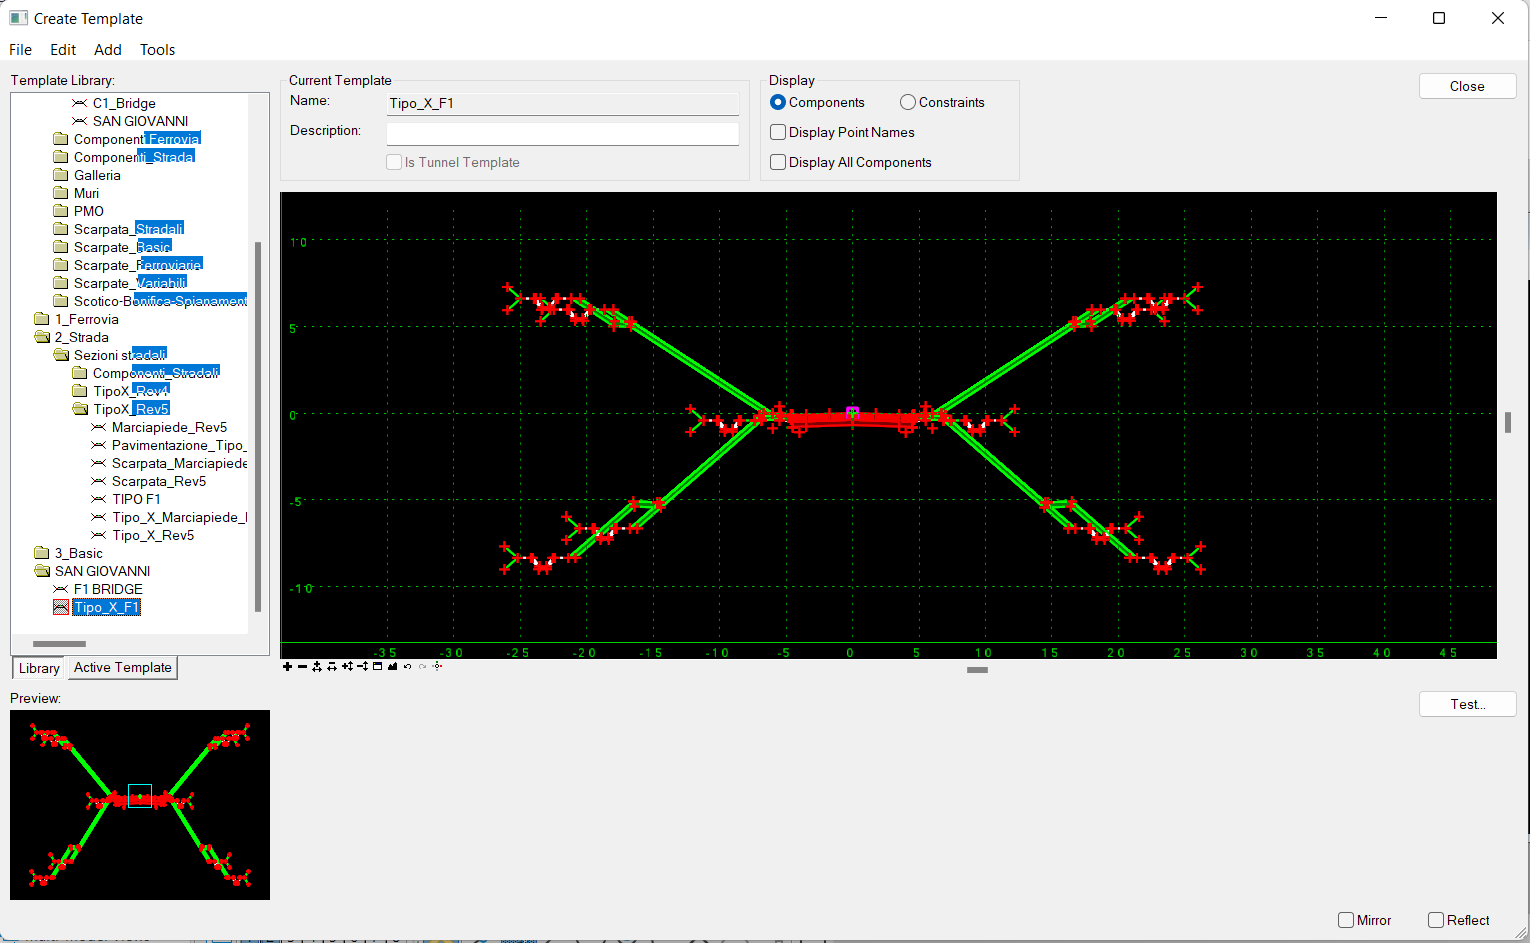
\includegraphics[width=\textwidth]{Figures/Sezione tipo X.png}
      \caption{Sezione tipo X}
      \label{Sezione tipo X}
\end{figure}

Per il nostro tracciato stradale è necessario anche l'inserimento di un'opera d'arte maggiore. Il procedimento è sempre lo stesso. Utilizziamo il comando Corridors/Create Template e selezioniamo in questo caso il template esistente $C1_BRIDGE$ adattandolo alla nostra tipologia di strada.

\begin{figure}[H]
    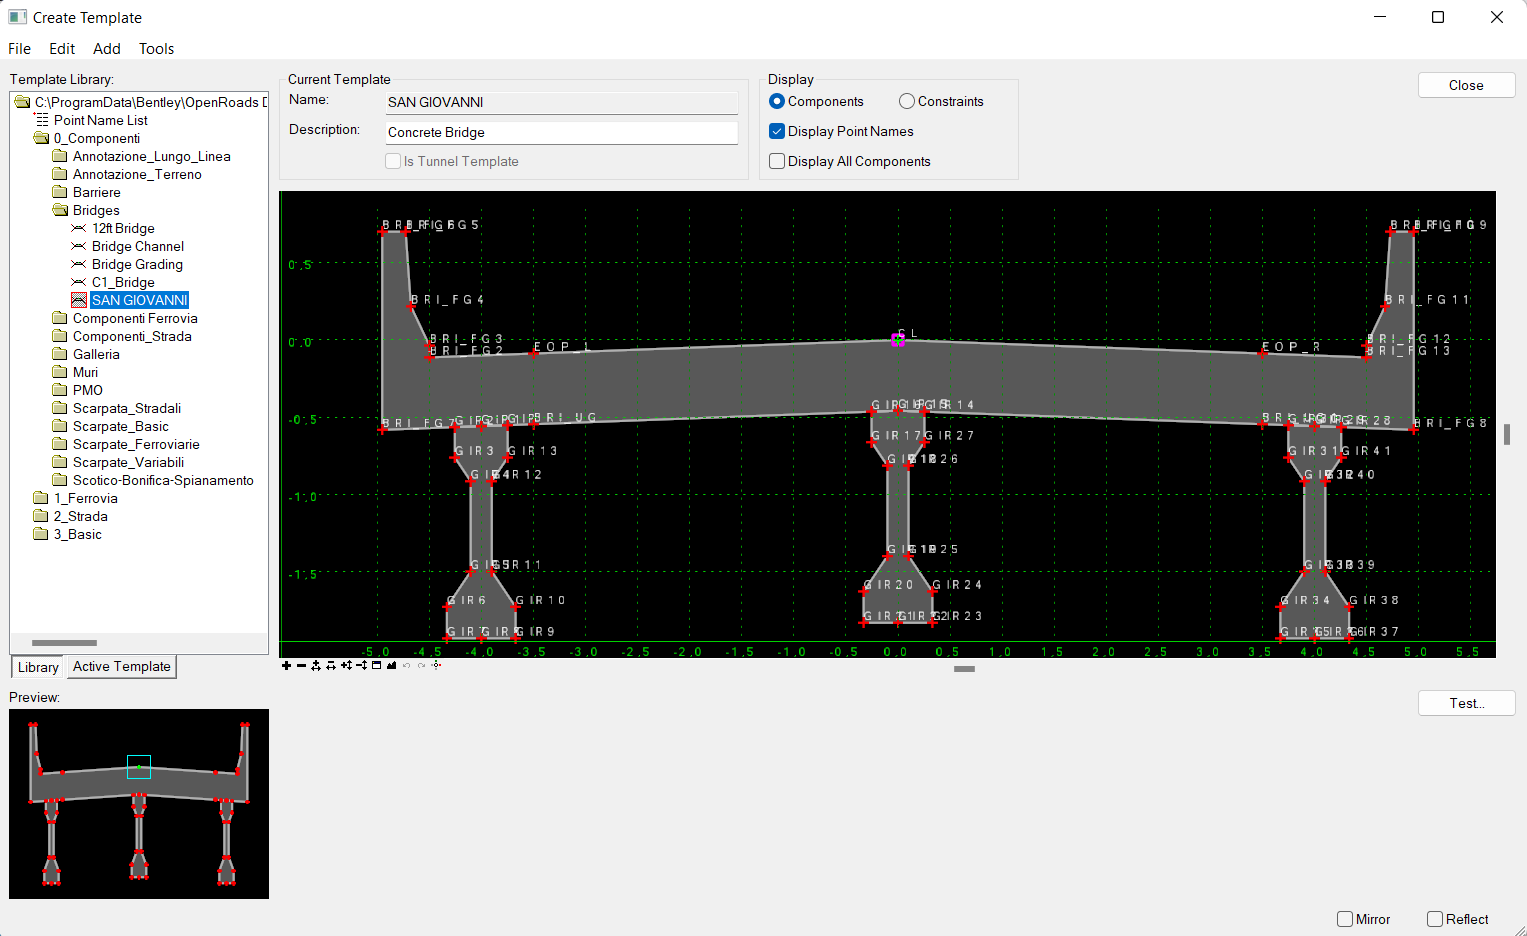
\includegraphics[width=\textwidth]{Figures/Sezione Bridge.png}
      \caption{Sezione Bridge}
      \label{Sezione Bridge}
\end{figure}

Possiamo creare un nuovo corridors. Per fare ciò si utilizza il comando Corridors/New Corridor/locate Profile, si ottiene così il modello tridimensionale della nostra strada.

Per completare il progetto bisogna applicare la sopraelevazione alla sezione stradale attraverso il comando assign superelevetion to corridor.

A questo punto abbiamo ottenuto il nostro corpo stradale. Di seguito si riportano alcune viste differenti:

\begin{figure}[H]
    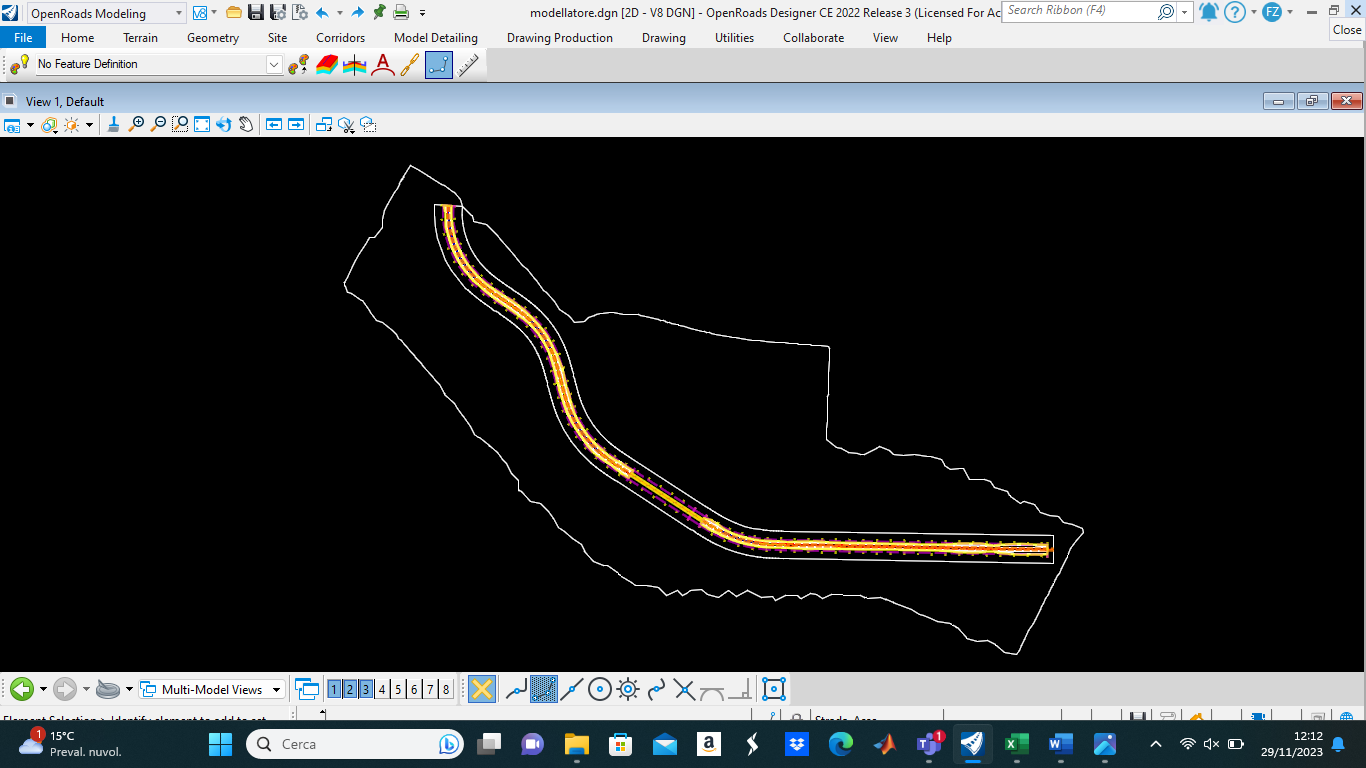
\includegraphics[width=\textwidth]{Figures/Vista piana in 2D.png}
      \caption{Vista piana in 2D}
      \label{Vista piana in 2D}
\end{figure}

\begin{figure}[H]
    \includegraphics[width=\textwidth]{Figures/Vista dall’alto 3D -1.png}
      \caption{Vista dall’alto 3D}
      \label{Vista dall’alto 3D}
\end{figure}

\begin{figure}[H]
    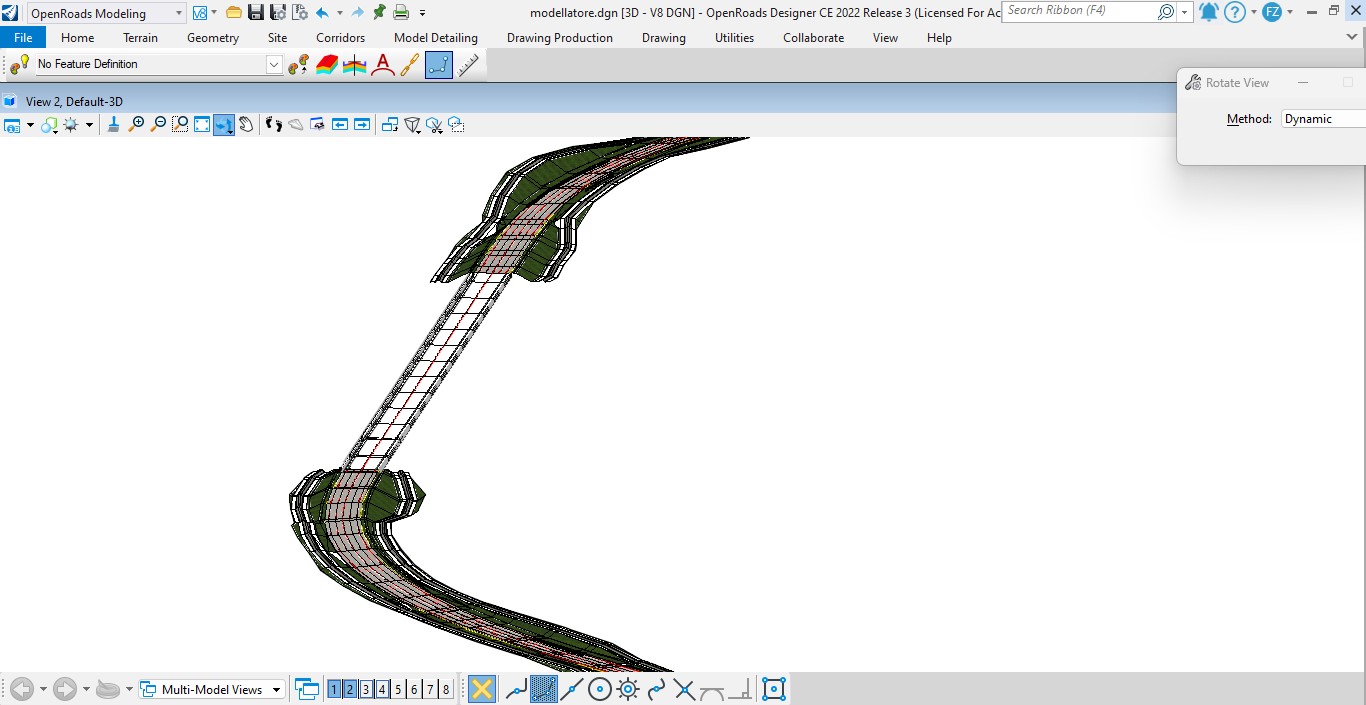
\includegraphics[width=\textwidth]{Figures/Vista in dettaglio 3D - 1.png}
      \caption{Vista in dettaglio 3D - 1}
      \label{Vista in dettaglio 3D - 1}
\end{figure}

\begin{figure}[H]
    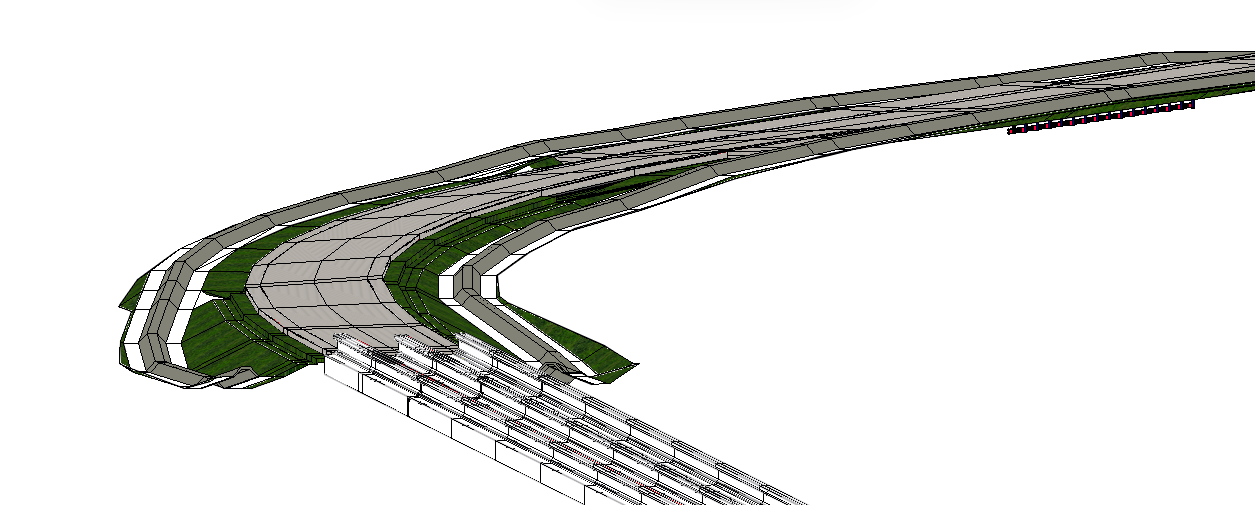
\includegraphics[width=\textwidth]{Figures/Vista in dettaglio 3D - 2.png}
      \caption{Vista in dettaglio 3D - 2}
      \label{Vista in dettaglio 3D - 2}
\end{figure}

\begin{figure}[H]
  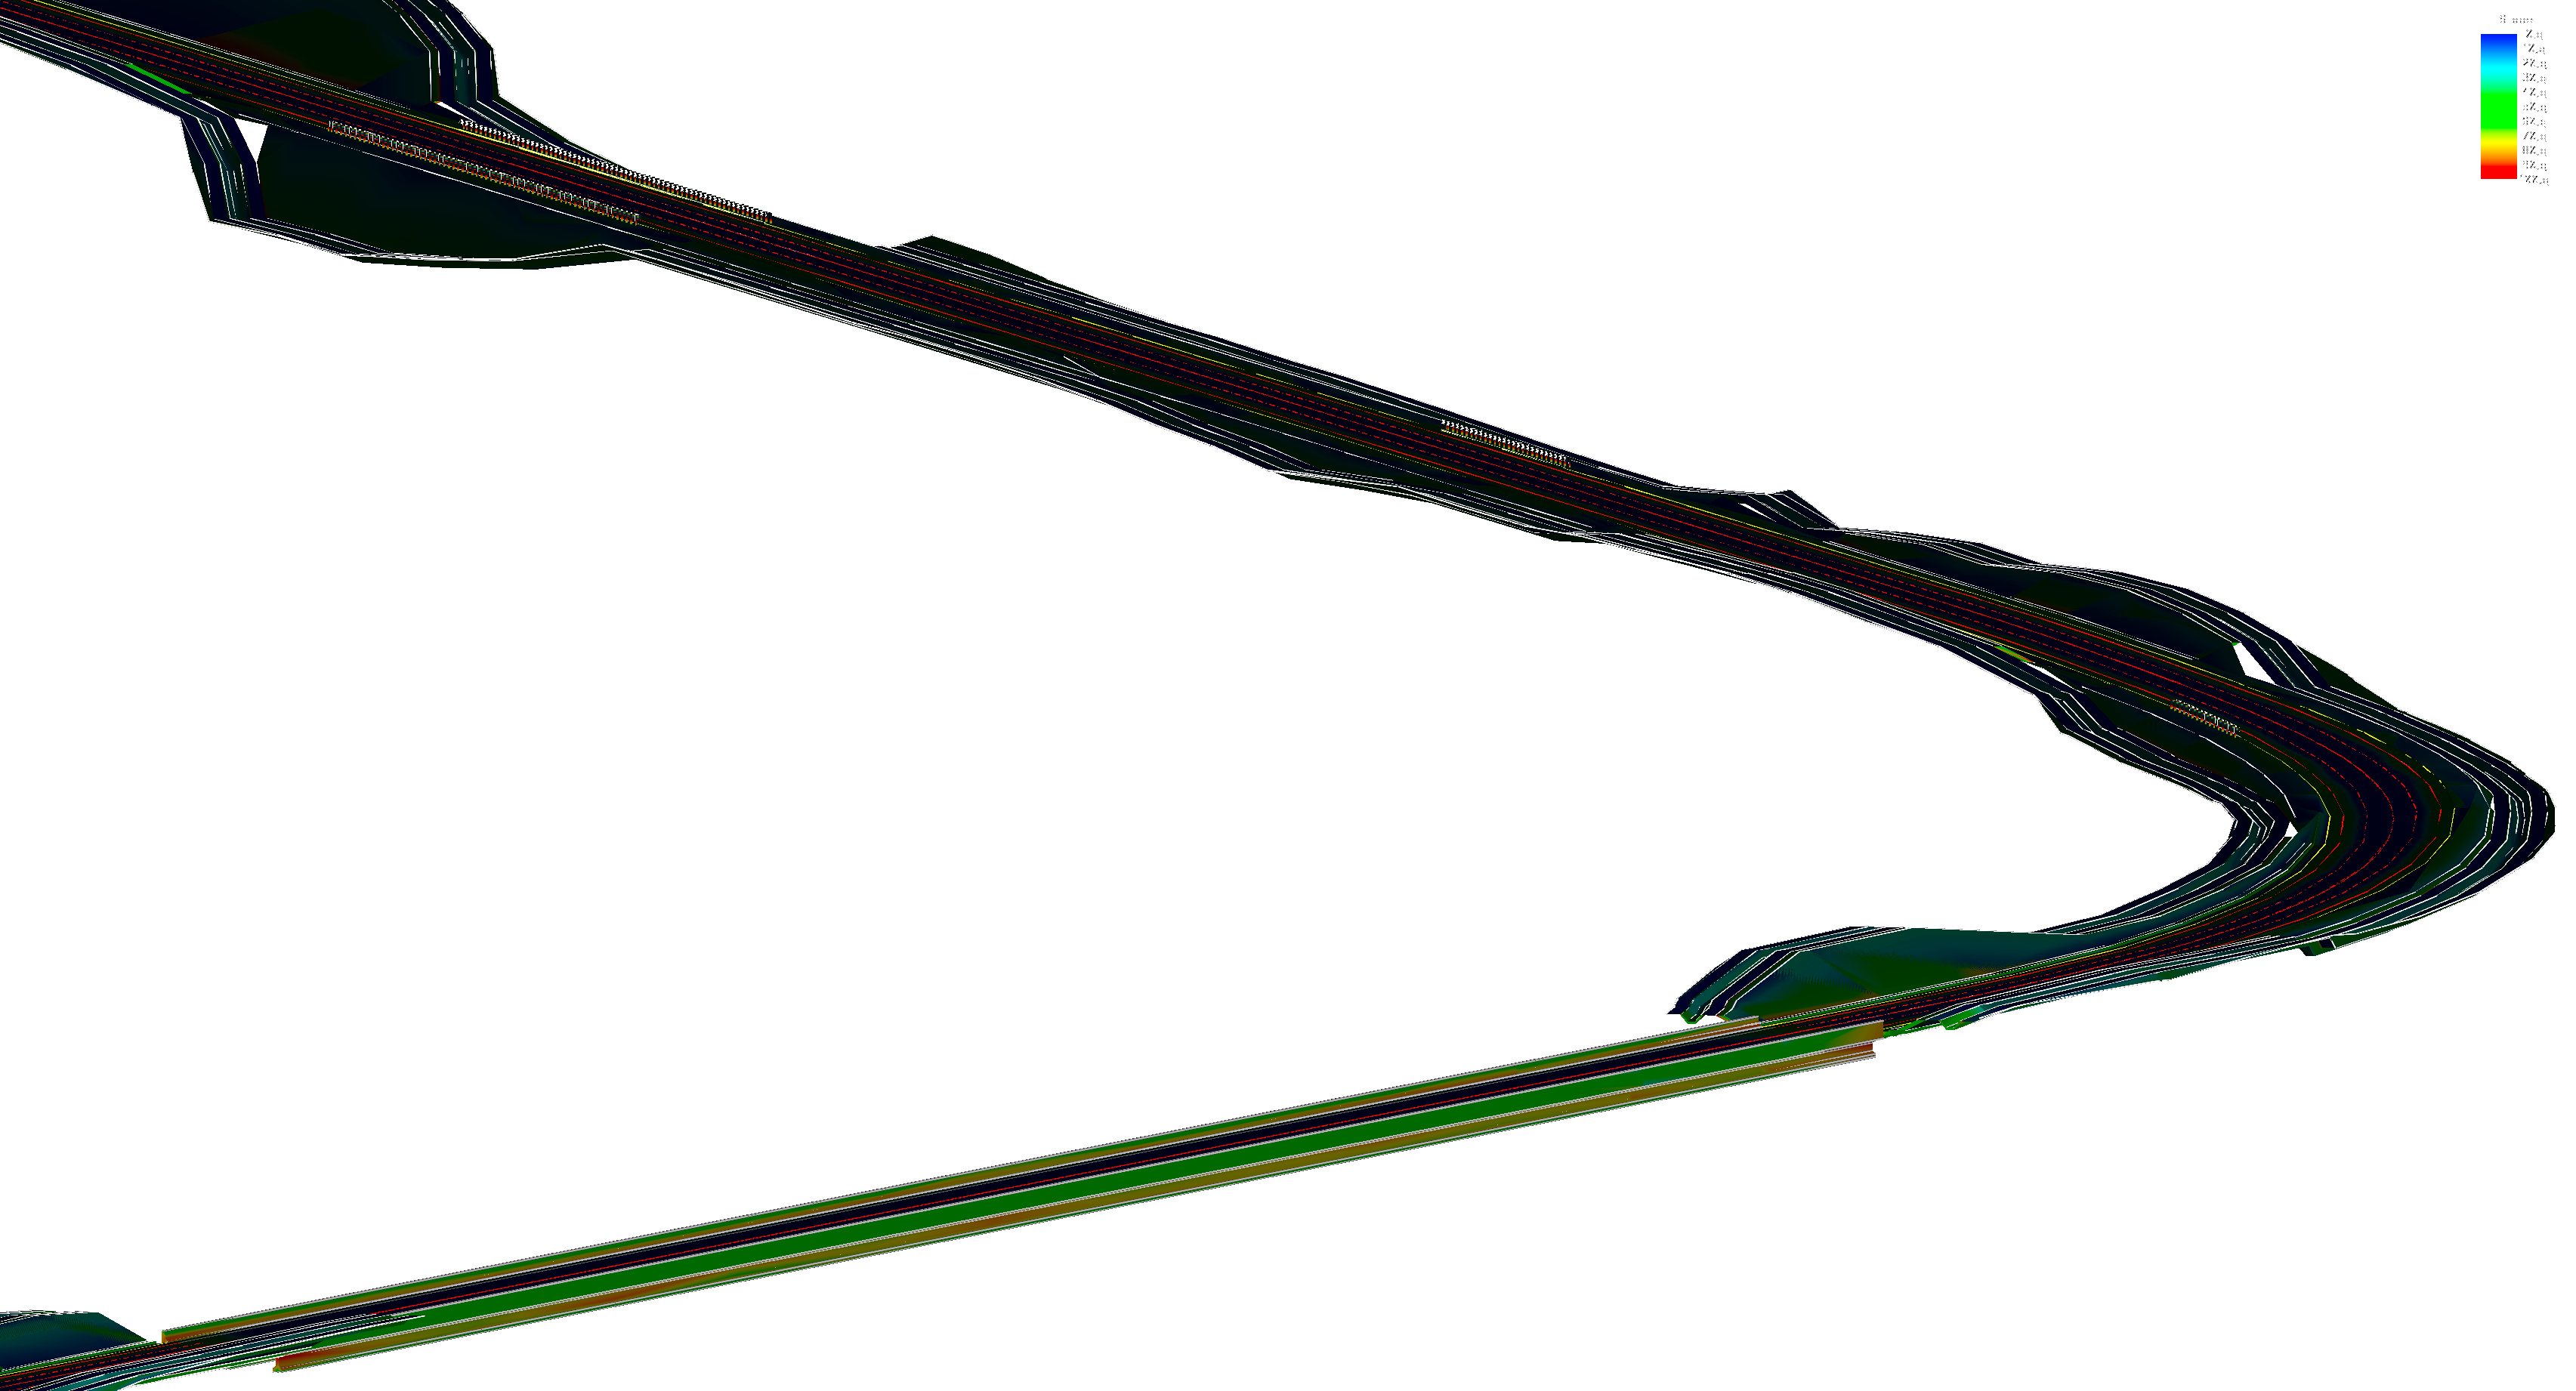
\includegraphics[width=\textwidth]{Figures/Vista in dettaglio 3D - 3.png}
    \caption{Vista in dettaglio 3D - 3}
    \label{Vista in dettaglio 3D - 3}
\end{figure}